\ifdefined\DISSERTATION
The LVars programming model presented in Chapter~\ref{ch:lvars} is
based on the idea of \emph{monotonic data structures}, in which
information can only be added, never removed, and the timing with
which information is added (and hence the \emph{order} in which it is
added) is not observable.  A paradigmatic example is a set that
supports insertion but not removal, but there are many others.  In the
LVars model, all shared data structures (called LVars) are monotonic,
and the states that an LVar can take on form a \emph{lattice}.  Writes
to an LVar must correspond to a lub operation in the lattice, which
means that they monotonically increase the information in the LVar,
and that they commute with one another.  But commuting writes are not
enough to guarantee determinism: if a read can observe whether or not
a concurrent write has happened, then it can observe differences in
scheduling.  So, in the LVars model, the answer to the question ``has
a write occurred?''  (\ie, is the LVar above a certain lattice value?)
is always
\emph{yes}; the reading thread will block until the LVar's contents
reach a desired threshold.  In a monotonic data structure, the absence
of information is transient---another thread could add that
information at any time---but the presence of information is forever.
\fi

We want to use LVars to implement fixpoint computations like the
parallel graph traversal of Section~\ref{s:lvars-motivation}.  But we
cannot do so using only least-upper-bound writes and threshold reads,
because in order to determine when the set of traversed nodes in the
graph has reached a fixpoint, we need to be able to see the exact
contents of that set, and it is impossible to learn the exact contents
of the set using only threshold reads.

\ifdefined\DISSERTATION
\begin{wrapfigure}{l}{2.5in}
\vspace{-1em}
\begin{center}
  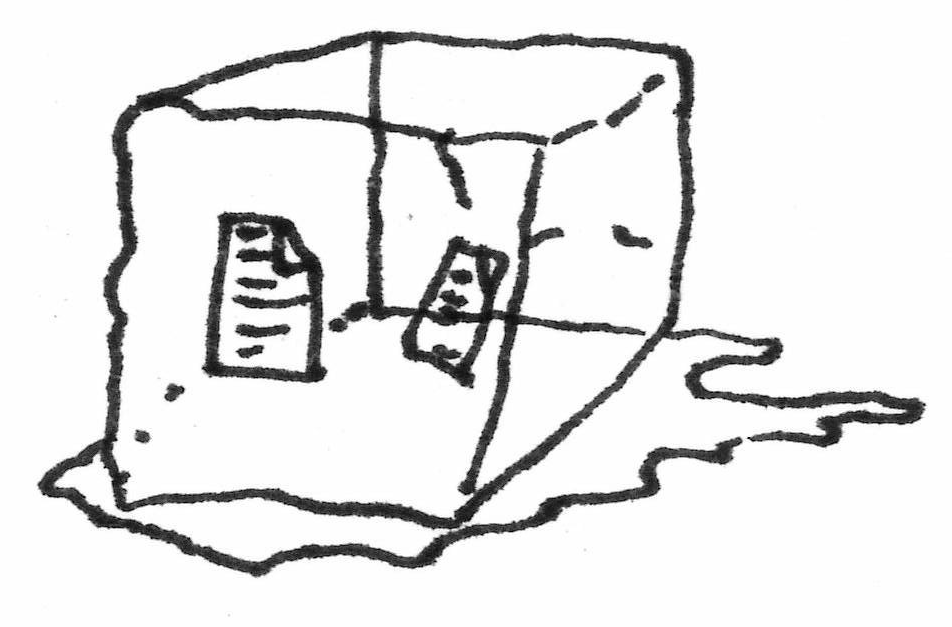
\includegraphics[scale=0.15]{../illustrations/frozen-data}
\end{center}
\vspace{-1em}
\end{wrapfigure}
\fi

In this \either{chapter, I}{section, we} describe two extensions to the basic LVars model
of \either{Chapter}{Section}~\ref{ch:lvars} that give us a new way to approach problems like
the parallel graph traversal problem.
First, \either{I}{we} add the ability to attach \emph{event handlers} to an LVar
that allow callback functions to run in response to updates to
the LVar.  We say that a group of event handlers is \emph{quiescent} when no callbacks
are currently enabled to run.  Second, \either{I}{we} add a new primitive
operation, @freeze@, that returns the exact contents of an LVar
without blocking.  Using @freeze@ to read an LVar comes with the
following tradeoff: once an LVar has been read, it is \emph{frozen},
and any further writes that would change its value instead throw an
exception.

The threshold reads that we have seen so far encourage a
synchronous, \emph{pull} model of programming in which threads ask
specific questions of an LVar, potentially blocking until the answer
is ``yes''.  The addition of handlers, quiescence, and freezing, by contrast, enables
an asynchronous, \emph{push} model of programming.  We will refer to
this extended programming model as the \emph{LVish} programming model.  Because quiescence
makes it possible to tell when the fixpoint of a computation has been
reached, the LVish model is particularly well suited to problems like
the graph traversal problem that we saw in
Section~\ref{s:lvars-motivation}.

Unfortunately, freezing does not commute with writes that change an
LVar.\footnote{The same is true for quiescence detection, as we will see in
Section~\ref{subsection:quasi-quiescence}.}  If a freeze is
interleaved before such a write, the write will raise an exception; if
it is interleaved afterwards, the program will proceed normally.  It
would appear that the price of negative information is the loss of
determinism!

Fortunately, the loss is not total.  Although LVar programs with
freezing are not guaranteed to be deterministic, they do satisfy a
related property that \either{I}{we} call \emph{quasi-determinism}: all executions
that produce a final value produce the \emph{same} final value.  To
put it another way, a quasi-deterministic program can be trusted to
never change its answer due to nondeterminism; at worst, it might
raise an exception on some runs.  This exception can in principle
pinpoint the exact pair of freeze and write operations that are
racing, greatly easing debugging.

In general, the ability to make exact observations of the contents of
data structures is in tension with the goal of guaranteed determinism.
Since pushing towards full-featured, general monotonic data structures
leads to flirtation with nondeterminism, perhaps the best way of
ultimately getting deterministic outcomes is to traipse a short
distance into nondeterministic territory, and make our way back.  The
identification of quasi-deterministic programs as a useful
intermediate class of programs is a contribution of \either{this dissertation}{our work}.
That said, in many cases the @freeze@ construct is only used as the
very final step of a computation: after a global barrier, freezing is
used to extract an answer.  In this common case, determinism is
guaranteed, since no writes can subsequently occur.

\either{I}{We} will refer to the LVars model, extended with handlers, quiescence,
and freezing, as the \emph{LVish model}.  The rest of this \either{chapter}{section} introduces
the LVish programming model, first informally through a series of examples, and then formally, by extending
the $\lambdaLVar$ calculus of \either{Chapter}{Section}~\ref{ch:lvars} to add support
for handlers, quiescence, freezing, and the arbitrary update operations described in
Section~\either{\ref{subsection:lvars-generalizing-from-least-upper-bound-writes}}{\ref{s:lvars-generalizing}}, resulting in a calculus \either{I}{we} call $\lambdaLVish$.
\either{I}{We} will also return to our parallel graph traversal problem and show
an solution implemented using the LVish Haskell library.

Finally, the main technical result of this \either{chapter}{section}
is a proof of quasi-determinism for $\lambdaLVish$. The key to the
proof is a generalized version of the Independence lemma
of \either{Chapter}{Section}~\ref{ch:lvars} that accounts for both
freezing and the arbitrary update operations that $\lambdaLVish$
allows.
